% This is LLNCS.DEM the demonstration file of
% the LaTeX macro package from Springer-Verlag
% for Lecture Notes in Computer Science,
% version 2.3 for LaTeX2e



\documentclass{llncs}


\usepackage{ngerman}
\usepackage[T1]{fontenc}
\usepackage[utf8]{inputenc}
\usepackage{makeidx}  % allows for indexgeneration
\usepackage{multirow}
\usepackage{rotating}
\usepackage{verbatim}
\usepackage{graphicx}
\usepackage{float}
\usepackage{amssymb}   % AMS-Sonderzeichen
\usepackage{tabularx}  % Für tabularx und newcolumntype
\usepackage[paper=a4paper,left=25mm,right=25mm,top=25mm,bottom=25mm]{geometry}
\usepackage{array}
\usepackage{makecell}
\usepackage{color}
\usepackage{ragged2e}
\usepackage{ifpdf}
% \usepackage{titlesec}
\usepackage{xcolor}    % Lieber xcolor als color. Dann klappt auch das listings gut mit den Farben
\usepackage{listings}
\usepackage{upquote}   % Verändert die Ausgabe der einfachen Anführungszeichen innerhalb von verbatim
\usepackage{eurosym}   % Euro-Zeichen: \euro
\usepackage{lastpage}  % \pageref{LastPage} um die Anzahl der Seiten zu erhalten
% hiermit kann man auch umlaute copy-pasten
\usepackage{lmodern}
\selectlanguage{english}
\usepackage{fancyhdr}
\usepackage{url}
\usepackage{caption}
\usepackage{float}
\setlength{\abovecaptionskip}{0pt} % Reduce space above the caption
\setlength{\belowcaptionskip}{0pt} % Space between caption and table
\captionsetup[table]{skip=5pt} % Adjust the value of '10pt' as needed
\pagestyle{fancy}
% Reduce space between float and surrounding text
\setlength{\textfloatsep}{0pt}
\setlength{\floatsep}{0pt}
\setlength{\intextsep}{0pt}



%

\ifpdf
\pdfinfo{
   /Author (Wladymir Alexander Brborich Herrera)
   /Author (Vishwaben Pareshbhai Kakadiya)
   /Author (Hellyben Bhaveshkumar Shah)
   /Author (Heer Rakeshkumar Vankawala)
   /Author (Priyanka Dilipbhai Vadiwala)
   /Title  (LowTech GMmBH Techincal Transformation Milestone 2)
   /Subject (Cloud Computing)
   /Keywords (Cloud Computing, Technical Transformation, Migration)
}
\fi

\setlength{\parindent}{0pt}    % Erste Zeile eines Absatzes nicht einrücken
\parskip2ex                    % Absatzabstand
\setlength{\itemsep}{0ex plus0.2ex}
\sloppy                        % Auf jeden Fall die Seitenränder einhalten.

\newcommand{\what}{Milestone 2 : LowTech GMmBH Migration to Azure}
\newcommand{\who}{Group 23}
\newcommand{\when}{WiSe 2024-2025}

\renewcommand{\headrulewidth}{0.4pt}
\renewcommand{\footrulewidth}{0.4pt}
\lhead[\when]{\who}
\rhead[\who]{\when}
\chead[]{}
\lfoot[Page \thepage\ of \pageref{LastPage}]{\what}
\rfoot[\what]{Page \thepage\ of \pageref{LastPage}}
\cfoot[]{}
\pagestyle{fancy}


% Hurenkinder und Schusterjungen komplett verbieten.
\clubpenalty = 10000 
\widowpenalty = 10000 
\displaywidowpenalty = 10000
% Diese Begriffe bezeichnen den Makel beim Textsatz, wenn eine Seite mit der ersten Zeile eines Absatzes endet (so genannter Schusterjunge) oder eine neue Seite mit der letzten Zeile eines Absatzes beginnt (so genanntes Hurenkind).


% Wir definieren ein paar Farben
\definecolor{Brown}{cmyk}{0,0.81,1,0.60}
\definecolor{OliveGreen}{cmyk}{0.64,0,0.95,0.40}
\definecolor{CadetBlue}{cmyk}{0.62,0.57,0.23,0}
\definecolor{lightlightgray}{gray}{0.9}
\definecolor{FrankfurtBlue}{HTML}{3333b2}

% Hier fängt das Dokument an!
\begin{document}

%
% \frontmatter          % for the preliminaries
%
% \tableofcontents
%
\mainmatter              % start of the contributions
%
\title{\what}
%
\author{
    Wladymir Alexander Brborich Herrera (1437876)\\
    \texttt{wladymir.brborich-herrera@stud.fra-uas.de}
    \and\\
    Vishwaben Pareshbhai Kakadiya (1471845)\\
    \texttt{vishwaben.kakadiya@stud.fra-uas.de}
    \and\\
    Hellyben Bhaveshkumar Shah (1476905)\\
    \texttt{hellyben.shah@stud.fra-uas.de}
    \and\\
    Heer Rakeshkumar Vankawala (1449039)
    \\
    \texttt{heer.vankawala@stud.fra-uas.de}
    \and\\
    Priyanka Dilipbhai Vadiwala (1481466)\\
    \texttt{priyanka.vadiwala@stud.fra-uas.de}
}
%
\institute{
    Frankfurt University of Applied Sciences\\
    (1971-2014: Fachhochschule Frankfurt am Main)\\
    Nibelungenplatz 1\\
    D-60318 Frankfurt am Main\\
}

\maketitle              % typeset the title of the contribution

\begin{abstract}

\end{abstract}

\section{Overview of the Problem}


\section{Objectives of the Migration}

\section{Migration Strategy}

After reviewing the company landscape we have evaluated several options for the migration to a public/private cloud context depending on the application.
For each one we detail the Cloud Context to deploy, which tools to use, and, if relevant, details on the service models of each product.

\subsection{Finance: Legacy Application}

As the finance department still needs to use this application for the next 3 years, we are only going to migrate to our own private cloud context.
In this case, it is going to be deployed into a virtual machine with the ability to scale in terms of memory and CPU thanks to PoxMox.
For backup purposes, we will create a file share specific to this application using Azure Files.
We are also going to use Ansible playbooks to automate the configuration and installation of the application.\\

\begin{table}[h!]
    \centering
    \begin{tabular}{lll}
        \hline
        \textbf{Cloud Context} & \textbf{Products And Technologies} & \textbf{Service Models} \\
        \hline
        Private Cloud          & ProxMox, Ansible                   & N/A                     \\
        \hline
        Public Cloud           & Azure Files                        & IaaS                    \\
        \hline
    \end{tabular}
    \caption{Finance Legacy Application Deployment Strategy}
\end{table}


\subsection{Finance: SAP PPM, ERP, IAM and ERM}
These applications will also be deployed in the new private cloud context.
Since the finance department is the only one that needs access, this system will be somewhat isolated.
We are going to configure networking access only for the finance department clients.
Following the same patterns as for the Legacy application, we are also going to use Ansible to automate and make the installation and configuration repeatable.\\


\begin{table}[h!]
    \centering
    \begin{tabular}{lll}
        \hline
        \textbf{Cloud Context} & \textbf{Products And Technologies} & \textbf{Service Models} \\
        \hline
        Private Cloud          & ProxMox, Ansible                   & N/A                     \\
        \hline
    \end{tabular}
    \caption{Finance SAP PPM, ERP, IAM and ERM Deployment Strategy}
\end{table}

\subsection{Production: Reporting Management}
This application will be newly developed, for this, we are going to deploy the backend using Azure App Service, the front end using Azure Static Web Apps, Azure Blob Storage to save reports, and Azure CosmosDB if a database is needed.
To secure all newly developed applications we are going to use Microsoft Entra ID, and make them accessible only with the company VPN.\\
\begin{table}[h!]
    \centering
    \begin{tabular}{lll}
        \hline
        \textbf{Cloud Context} & \textbf{Products And Technologies} & \textbf{Service Models} \\
        \hline
        Public Cloud           & Azure App Service                  & PaaS or CaaS            \\
        \hline
        Public Cloud           & Azure Static Web App               & PaaS or CaaS            \\
        \hline
        Public Cloud           & Azure Blob Storage                 & IaaS                    \\
        \hline
        Public Cloud           & Microsoft Entra ID                 & PaaS                    \\
        \hline
        Public Cloud           & Azure Cosmos DB                    & PaaS                    \\
        \hline
    \end{tabular}
    \caption{Production Reporting Management Deployment Strategy}
\end{table}


\subsection{Production + HR: Shift Management}
This application will be newly developed. Following the standard for new applications, we will deploy the backend using Azure App Service, the front end using Azure Static Web Apps, and Azure Database For PostgreSQL if a database is needed.
To secure all newly developed applications we are going to use Microsoft Entra ID, and make them accessible only with the company VPN.\\

\begin{table}[h!]
    \centering
    \begin{tabular}{lll}
        \hline
        \textbf{Cloud Context} & \textbf{Products And Technologies} & \textbf{Service Models} \\
        \hline
        Public Cloud           & Azure App Service                  & PaaS or CaaS            \\
        \hline
        Public Cloud           & Azure Static Web App               & PaaS or CaaS            \\

        \hline
        Public Cloud           & Microsoft Entra ID                 & PaaS                    \\
        \hline
        Public Cloud           & Azure Database For PostgreSQL      & PaaS                    \\
        \hline
    \end{tabular}
    \caption{Production, HR, Shift Management Deployment Strategy}
\end{table}

\subsection{Supply Management: SCM}
This application is supplied by a third party. It will be installed in a linux virtual machine, using Azure Linux Virtual Machines + Azure Virtual Machine Scale Sets, to enable autoscaling.
Same as all other internal applications, it will only be accessible through the company VPN.\\

\begin{table}[h!]
    \centering
    \begin{tabular}{lll}
        \hline
        \textbf{Cloud Context} & \textbf{Products And Technologies}                              & \textbf{Service Models} \\
        \hline
        Public Cloud           & Azure Linux Virtual Machines + Azure Virtual Machine Scale Sets & IaaS                    \\
    \end{tabular}
    \caption{Supply Management SCM Deployment Strategy}
\end{table}

\subsection{Quality Management: QM Software}
This application is supplied by a third party. It will be installed in a windows virtual machine, using Azure Windows Virtual Machines + Azure Virtual Machine Scale Sets, to enable autoscaling.
Same as all other internal applications, it will only be accessible through the company VPN.\\

\begin{table}[h!]
    \centering
    \begin{tabular}{lll}
        \hline
        \textbf{Cloud Context} & \textbf{Products And Technologies}                                & \textbf{Service Models} \\
        \hline
        Public Cloud           & Azure Windows Virtual Machines + Azure Virtual Machine Scale Sets & IaaS                    \\
    \end{tabular}
    \caption{Quality Management QM Software Deployment Strategy}
\end{table}

\subsection{Warehouse: Warehouse Management}
This application will be newly developed. Following the standard for new applications, we will deploy the backend using Azure App Service, the front end using Azure Static Web Apps, and Azure Database For PostgreSQL if a database is needed.
To secure all newly developed applications we are going to use Microsoft Entra ID, and make them accessible only with the company VPN.\\

\begin{table}[h!]
    \centering
    \begin{tabular}{lll}
        \hline
        \textbf{Cloud Context} & \textbf{Products And Technologies} & \textbf{Service Models} \\
        \hline
        Public Cloud           & Azure App Service                  & PaaS or CaaS            \\
        \hline
        Public Cloud           & Azure Static Web App               & PaaS or CaaS            \\

        \hline
        Public Cloud           & Microsoft Entra ID                 & PaaS                    \\
        \hline
        Public Cloud           & Azure Database For PostgreSQL      & PaaS                    \\
        \hline
    \end{tabular}
    \caption{Warehouse, Warehouse Management}
\end{table}

\subsection{Warehouse: Deliforce}

This application will be installed on premise. As other on premise deployments we will automate it with Ansible.
It will communicate with other internal applications using Azure Express Route, enabling us to transfer information between our private cloud and its public counterpart.\\

\begin{table}[h!]
    \centering
    \begin{tabular}{lll}
        \hline
        \textbf{Cloud Context} & \textbf{Products And Technologies} & \textbf{Service Models} \\
        \hline
        Public Cloud           & Azure Express Route                & PaaS                    \\
        \hline
        Private Cloud          & ProxMox, Ansible                   & N/A                     \\
        \hline
    \end{tabular}
    \caption{Warehouse Deliforce Deployment Strategy}
\end{table}

\subsection{Sales + Operations + Customer Service: CRM}

This application is supplied by a third party. It will be installed in a linux virtual machine, using Azure Linux Virtual Machines + Azure Virtual Machine Scale Sets, to enable autoscaling.
As all other internal applications, it will only be accessible through the company VPN.\\

\begin{table}[h!]
    \centering
    \begin{tabular}{lll}
        \hline
        \textbf{Cloud Context} & \textbf{Products And Technologies}                              & \textbf{Service Models} \\
        \hline
        Public Cloud           & Azure Linux Virtual Machines + Azure Virtual Machine Scale Sets & IaaS                    \\
    \end{tabular}
    \caption{Quality Management QM Software Deployment Strategy}
\end{table}

\subsection{Sales: Lead Management}
This application will be installed on premise. As other on premise deployments we will automate it with Ansible.
\begin{table}[h!]
    \centering
    \begin{tabular}{lll}
        \hline
        \textbf{Cloud Context} & \textbf{Products And Technologies} & \textbf{Service Models} \\
        \hline
        Private Cloud          & ProxMox, Ansible                   & N/A                     \\
        \hline
    \end{tabular}
    \caption{Sales Lead Management Deployment Strategy}
\end{table}

\subsection{Sales: Business Analytics}
This application is supplied by a third party. It will be installed in a linux virtual machine, using Azure Linux Virtual Machines + Azure Virtual Machine Scale Sets, to enable autoscaling.
As all other internal applications, it will only be accessible through the company VPN.\\

\begin{table}[h!]
    \centering
    \begin{tabular}{lll}
        \hline
        \textbf{Cloud Context} & \textbf{Products And Technologies}                              & \textbf{Service Models} \\
        \hline
        Public Cloud           & Azure Linux Virtual Machines + Azure Virtual Machine Scale Sets & IaaS                    \\
    \end{tabular}
    \caption{Sales Business Analytics Deployment Strategy}
\end{table}

\subsection{Sales: Tableu (Market Development)}
This application is supplied by a third party. It will be installed in a custom virtual machine, using Azure Tableu Server.
In this case we are not going to actively enable auto scaling, since we anticipate that te use case does not benefit from adding more instances.
As other internal applications it will only be accessible through the company VPN.\\

\begin{table}[h!]
    \centering
    \begin{tabular}{lll}
        \hline
        \textbf{Cloud Context} & \textbf{Products And Technologies} & \textbf{Service Models} \\
        \hline
        Public Cloud           & Azure Tableu Server                & IaaS                    \\
        N/A                    & Tableu Desktop                     & N/A                     \\
    \end{tabular}
    \caption{Sales Tableu (Market Development) Deployment Strategy}
\end{table}

\subsection{HR: HR Software}
This application will be newly developed following the standard for new applications.
To secure all newly developed applications we are going to use Microsoft Entra ID, and make them accessible only with the company VPN.\\

\begin{table}[h!]
    \centering
    \begin{tabular}{lll}
        \hline
        \textbf{Cloud Context} & \textbf{Products And Technologies} & \textbf{Service Models} \\
        \hline
        Public Cloud           & Azure App Service                  & PaaS or CaaS            \\
        \hline
        Public Cloud           & Azure Static Web App               & PaaS or CaaS            \\

        \hline
        Public Cloud           & Microsoft Entra ID                 & PaaS                    \\
        \hline
        Public Cloud           & Azure Database For PostgreSQL      & PaaS                    \\
        \hline
    \end{tabular}
    \caption{HR Software Deployment Strategy}
\end{table}

\subsection{Facility Management: Facility Management Software}
This is a proprietary application that will be deployed on premises following practices stated for all previous on premise deployments\\
\begin{table}[h!]
    \centering
    \begin{tabular}{lll}
        \hline
        \textbf{Cloud Context} & \textbf{Products And Technologies} & \textbf{Service Models} \\
        \hline
        Private Cloud          & ProxMox, Ansible                   & N/A                     \\
        \hline
    \end{tabular}
    \caption{Facility Management Software Deployment Strategy}
\end{table}

\subsection{Finance + HR + Sales + Legislation: Office Suite}
In this case, several departments need access to the office suite. We are going to provide them with access to the Microsoft 365 selection of products.
Each client will have the option to use the office suite in the cloud, or locally on their devices. We will also provide OneDrive access for easy document sharing and collaboration.\\

\begin{table}[h!]
    \centering
    \begin{tabular}{lll}
        \hline
        \textbf{Cloud Context} & \textbf{Products And Technologies} & \textbf{Service Models} \\
        \hline
        Public Cloud           & Microsoft Office 365               & SaaS                    \\
        \hline
        Public Cloud           & OneDrive                           & SaaS                    \\
        \hline
    \end{tabular}
    \caption{Office Suite Deployment Strategy}
\end{table}

\subsection{Webshop: Website CMS}

This application will be newly developed following the standard for new applications.
As a special consideration, this application is the only public facing application which needs to handle customer requests.
Our standard for newly developed applications enable this critical piece of the business to easily scale and be secured with valid certificates with no extra configurations.\\

\begin{table}[h!]
    \centering
    \begin{tabular}{lll}
        \hline
        \textbf{Cloud Context} & \textbf{Products And Technologies} & \textbf{Service Models} \\
        \hline
        Public Cloud           & Azure App Service                  & PaaS or CaaS            \\
        \hline
        Public Cloud           & Azure Static Web App               & PaaS or CaaS            \\
        \hline
        Public Cloud           & Azure Database For PostgreSQL      & PaaS                    \\
        \hline
    \end{tabular}
    \caption{Webshop Website Deployment Strategy}
\end{table}

\subsection{General Considerations}

Importantly, for all newly developed applications we will:
\begin{itemize}
    \item Set up a private GitHub repository
    \item Set up GitHub actions to enable continues integration and continuous deployments in Azure
    \item Set up an infrastructure folder to hold terraform files. These files will define the infrastructure and will allow for easy repeatability
    \item Use Microsoft Entra ID in case authentication with the organization is needed
    \item Use Docker to package the applicaation with containers that will be deployed in Azure App Service in case of the backend, and Azure Static Web Apps in case of the frontend
\end{itemize}
For all aplications that will be deployed on premises:
\begin{itemize}
    \item Set up a private GitHub repository
    \item Create Ansible playbooks to make configuration and instalation in a VM repeatable
    \item In case the application needs to communicate with another aplication deployed in the public cloud we will use Azure Express Route to create a getaway.
\end{itemize}

For all applications that will be installed on the cloud and run in virtual machines:
\begin{itemize}
    \item Set up a private GitHub repository
    \item Create terraform files to define the infrastructure i.e the VM size and OS
    \item Create Ansible playbooks to make configuration and instalation in a VM repeatable
\end{itemize}

\section{Proposed Cloud Architecture \& Justfication of Used Service Models}
By considering the requirements of LowTech GmbH, we offer Hyrid Cloud Architecture as mentioned earlier in section 3 and illustrated in the figure \ref{Cloud_Architecture} below. According to the newly modified application landscape, each department's software components use suitable service model solutions (IaaS, PaaS, and SaaS) from public or private cloud service providers.

\begin{figure}[htbp]
    \begin{center}
      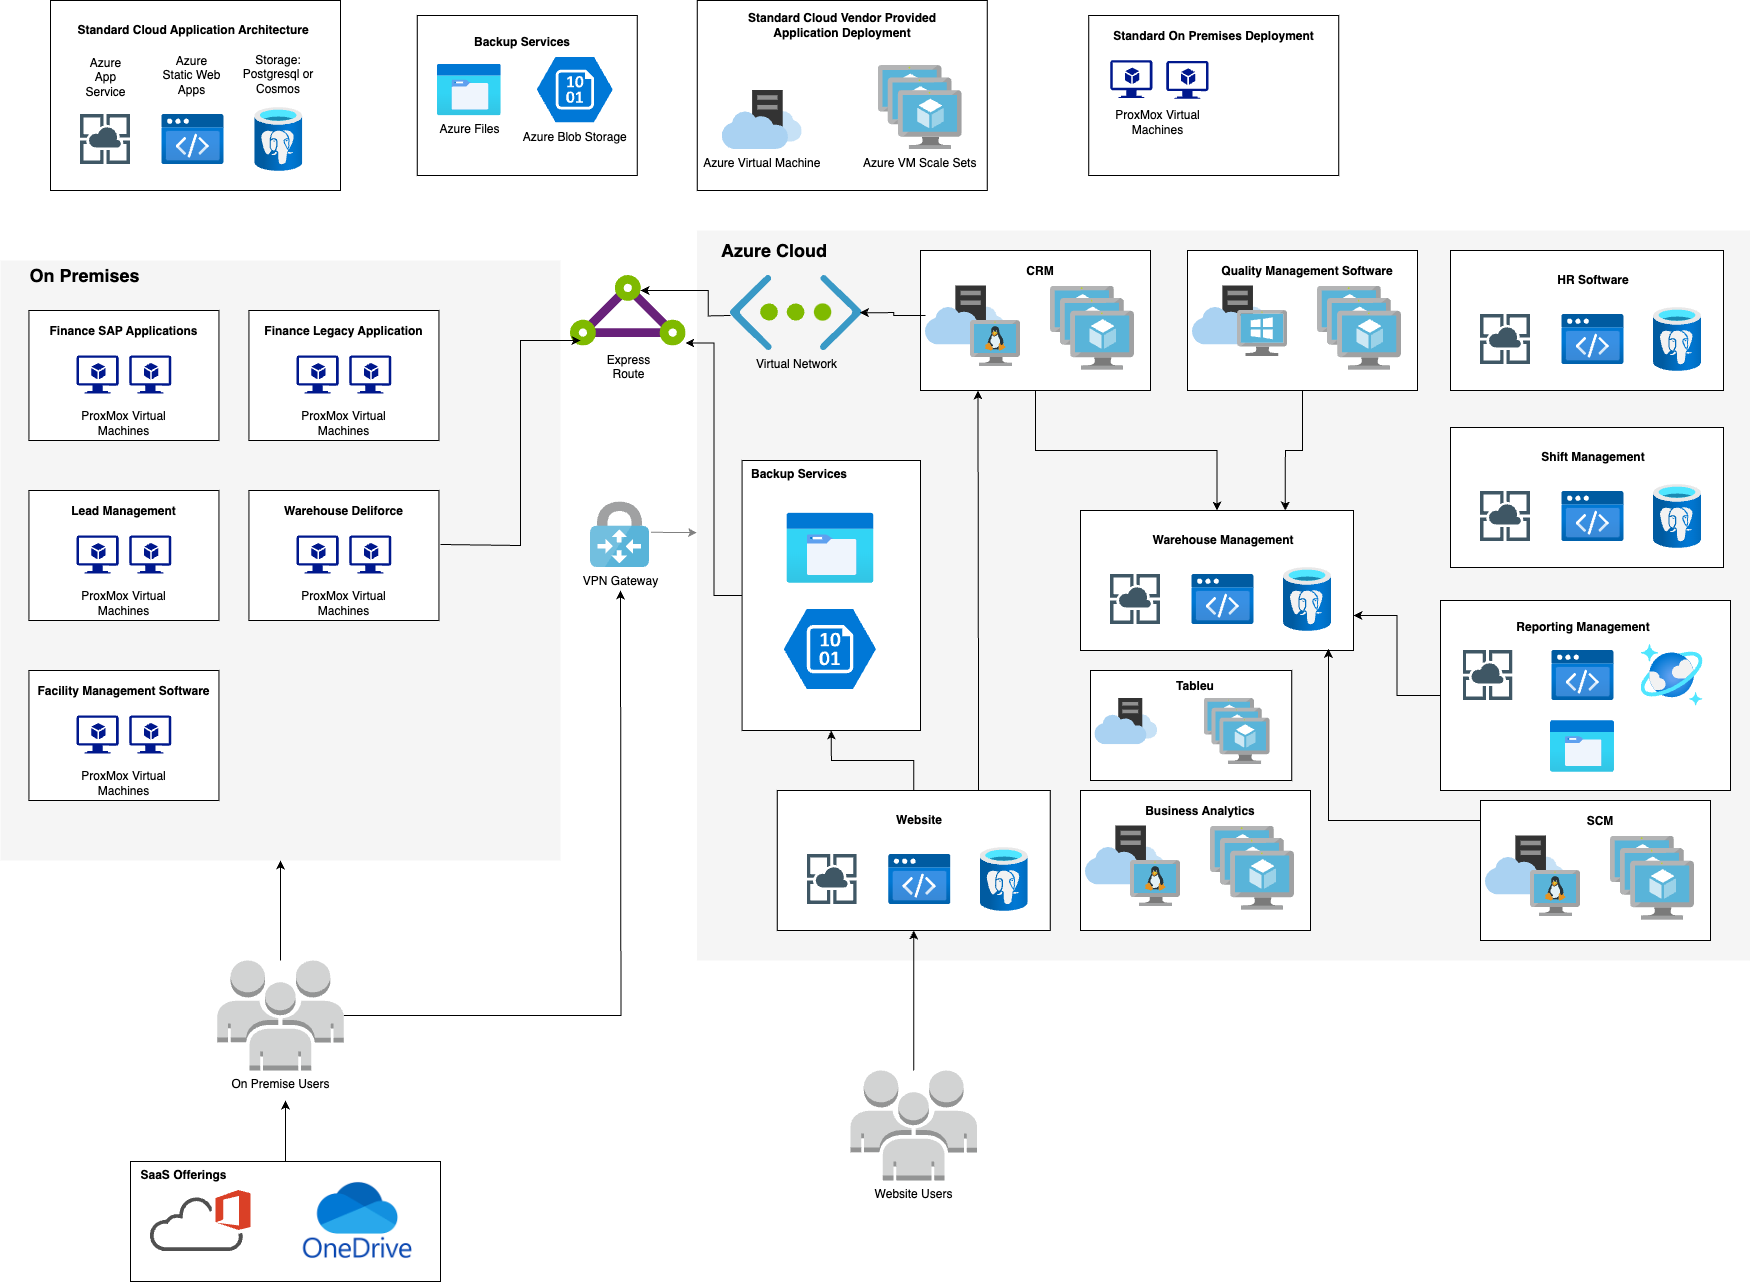
\includegraphics[width=1\textwidth]{diagrams/AzureArchCloud.png}
      \vspace{0.01\textwidth}
      \caption{Hybrid Cloud Architecture (Azure and On Premises)}
      \label{Cloud_Architecture} % A unique label.
    \end{center}
  \end{figure}

\subsection{Public Cloud Service Provider : Microsoft Azure}
\subsubsection{Azure App Serive: PaaS}
Azure App Service is a comprehensive Platform-as-a-Service (PaaS) offering for developers, providing a fully managed environment for building, deploying, and scaling web applications under offered service plan.

All the newly developed Python3 applications (Reporting Management,Shift Management, Warehouse Management, HR Software and Webshop Website) will be deployed within the single azure app service plan to optimize cost and performance, provided the plan has sufficient resources to handle the load as multiple apps in the same app Service plan share the same VM instances.

\begin{itemize}
    \item \textbf{Service Plan:} \textit{Premium v3}
    The premium service plan offers better compatibility with our application landscape and requirements compared to other tiers  due to following reasons.

    \begin{itemize}
        \item \textbf{Auto-scaling \& Per-app scaling} - With automatic scaling enabled, Azure will monitor the load on your apps and distribute instances based on the metrics set up as such CPU usage. It also supports per-app scaling, allowing each app to scale independently based on its specific load.
        \item \textbf{Availability \& Zone Redundancy} - Azure SLA guarantees 99.95\% availability but incase case of availability zone failures it is advised to configure app service plan as zone redundant,which means that your resources are spread across multiple availability zones. (Note: To enable zone-redundancy atleast 3 instances should be there in a app service plan).
        \item \textbf{Security} - Supports authentication, IP address restriction and also offer virtual network integration.
        \item \textbf{Load-balancing} - Distributes incoming traffic across multiple instances to maximize throughput, minimize response time, and avoid overloading any single resource.
        \item \textbf{Multi-tenant} - Multiple clients can access the solution via their own individual domains.
    \end{itemize}
    
    \item \textbf{Operating System:} \textit{Linux} - As Linux is the only operating system option for running Python apps in App Service. Linux is generally recommended due to better performance and compatibility with Python libraries1
    .Linux also offers a more native environment for Python development\cite{azure-python}.

    \item \textbf{VM Instance:} \textit{P2v3} - \#Instances: 3
    
    \begin{itemize}
        \item \textbf{Core:} \textit{4} 
        \item \textbf{RAM:} \textit{16} 
        \item \textbf{Storage:} \textit{250 GB} 
    \end{itemize}
\end{itemize}

\subsubsection{Azure Static Web App: PaaS}
\subsubsection{Microsoft Entra ID : PaaS}
\subsubsection{Azure Database(PostgreSQL/Cosmos DB) : PaaS}
\section{Cost of operations in Microsoft Azure}

\section{Migration Roadmap}



\section{Standard For a Cloud Native Application}


% ---- Bibliography ----

\begin{thebibliography}{5}

    \bibitem{MicrosoftAzureScaling}
    Microsoft,
    \emph{High-density hosting on Azure App Service using per-app scaling},
    2024,
    \url{https://learn.microsoft.com/en-us/azure/app-service/manage-scale-per-app}.

    
    \bibitem{MicrosoftAzureReliability}
    Microsoft,
    \emph{Reliability recommendations for Azure App Service},
    2024,
    \url{https://learn.microsoft.com/en-us/azure/reliability/reliability-app-service?pivots=premium}.
    
    \bibitem{MicrosoftAzureAppServiceOverviewDE}
    Microsoft,
    \emph{App Service-Übersicht},
    2024,
    \url{https://learn.microsoft.com/de-de/azure/app-service/overview}.
    
    \bibitem{MicrosoftAzureHostingPlans}
    Microsoft,
    \emph{Azure App Service plan overview},
    2024,
    \url{https://learn.microsoft.com/en-us/azure/app-service/overview-hosting-plans}.
    
    \bibitem{MicrosoftAzureSubscriptionLimits}
    Microsoft,
    \emph{Azure subscription and service limits, quotas, and constraints},
    2024,
    \url{https://learn.microsoft.com/en-us/azure/azure-resource-manager/management/azure-subscription-service-limits}.
    
    \bibitem{MicrosoftAzurePythonConfig}
    Microsoft,
    \emph{Configure Linux Python apps - Azure App Service},
    2024,
    \url{https://learn.microsoft.com/en-us/azure/app-service/configure-language-python}.
    


\end{thebibliography}
\end{document}
